\chapter{Concept and Design}
\label{cha:conceptanddesign}

Explain what defines our concept (setup):
\begin{itemize}
    \item Big picture setup explanation
    \item API format (RESTful JSON API)
    \item Client side vs. server side
    \item Authentication idea
    \item Database design
    \item etc...
\end{itemize}


\vspace{0.5cm}

\section{Big Picture}

As already mentioned our system will consist of two parts, the mobile clients side and the backend side which interconnectedly exchange data. The backend part itself is split up again in three parts of which one is an \enquote{external} (means: SNET) resource, the CYCLONE Federation Provider. This entity provides us with user management and session handling functionalities so that we are able to out source these tedious and error-prone tasks to them. On the other side CYCLONE profits from our experiences with its rather young service. Concerning our part of the backend side, the task was to serve two machines independently, the API server and the database server. This was expected to be achieved with Docker.

To gain an understanding of what system we were trying to build, the following image should be at help:

\begin{center}
    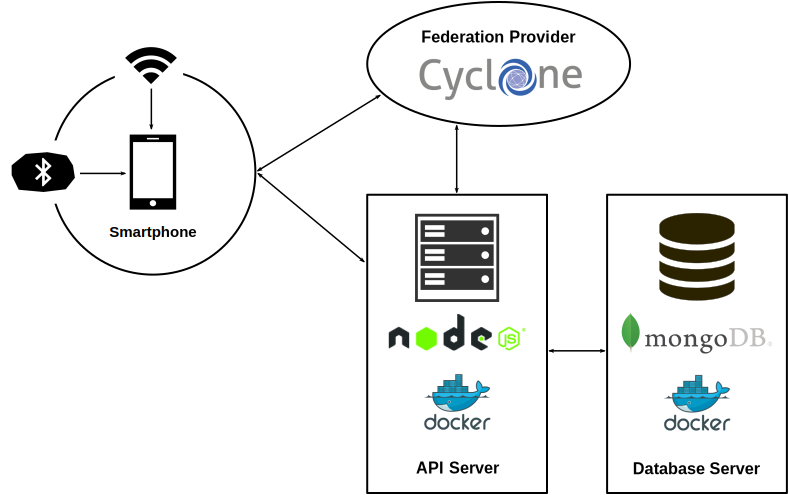
\includegraphics[width=\textwidth]{system-overview}\\
    All components of our envisioned system working together.
\end{center}

To sum it up, the idea is to gather position information aligned to the user's preferences locally on the smartphone, preform some processing steps on it, contact our backend for which authentication via the CYCLONE Federation Provider is needed and after that create, read, update or delete information (CRUD principle) in the backend and therefore in the database.


\vspace{0.5cm}

\section{API Considerations}

We had to decide on which paradigm our API should be based on. The client-server and stateless nature in combination with the just mentioned approach of relying on HTTP verbs such as POST, GET, PUT and DELETE for the CRUD operations, the decision to go for a RESTful API was quite clear (see chapter five \cite{fielding2000architectural}).


\vspace{0.5cm}

\section{Workload Split Between Clients and Server}


\vspace{0.5cm}

\section{Authentication and Session Management}


\vspace{0.5cm}

\section{Database Design}